\documentclass{article}
\usepackage{graphicx}
\usepackage{chemfig}
\usepackage{listings}
\usepackage{xcolor}
\usepackage{geometry} % Added package for adjusting margins

% Define custom colors for syntax highlighting
\definecolor{codegreen}{rgb}{0,0.6,0}
\definecolor{codegray}{rgb}{0.5,0.5,0.5}
\definecolor{codepurple}{rgb}{0.58,0,0.82}
\definecolor{backcolour}{rgb}{0.95,0.95,0.92}

\lstdefinestyle{mystyle}{
    backgroundcolor=\color{backcolour},
    commentstyle=\color{codegreen},
    keywordstyle=\color{magenta},
    numberstyle=\tiny\color{codegray},
    stringstyle=\color{codepurple},
    basicstyle=\ttfamily\small,
    breakatwhitespace=false,
    breaklines=true,
    captionpos=b,
    keepspaces=true,
    numbers=left,
    numbersep=5pt,
    showspaces=false,
    showstringspaces=false,
    showtabs=false,
    tabsize=2
}

\geometry{
  left=2.5cm,
  right=2.5cm,
  top=2.5cm,
  bottom=2.5cm
}

\lstset{style=mystyle}
\title{Lab 2}

\begin{document}

\begin{titlepage}
  \centering
  
\includegraphics[width=0.4\textwidth]{iithlogo.png}\par\vspace{1cm}
  {\scshape\LARGE Indian Institute of Technology Hyderabad \par}
  \vspace{1cm}
  {\scshape\Large Bioinformatics\par}
  \vspace{1.5cm}
\end{titlepage}

\maketitle
\newpage
\section{\textit{Mechanotransduction}}
Mechanotransduction, in cellular biology, refers to the diverse mechanisms by which cells convert mechanical stimuli (forces, pressure, etc.) into biochemical and electrical responses, influencing various cellular processes like growth, differentiation, and communication.
\subsection{Role played by Mechanotransduction in stem cell differentiation }
\begin{enumerate}
\item Sensing the Environment: Stem cells possess mechanosensors on their surface and within their cytoskeleton that detect mechanical changes

\item Signal Transduction: Upon sensing a force, the mechanosensors activate intricate signaling pathways within the cell. T which translate the mechanical signal into changes in gene expression and protein activity.

\item Directing Differentiation: The activated signaling pathways ultimately influence the expression of genes associated with specific cell lineages. 
\item For example, rigid substrates tend to promote osteogenic differentiation (bone cells), while softer substrates favor adipogenic differentiation (fat cells).
\end{enumerate}
\section{\textit{Research Papers}}
\subsection{Mechanotransduction in Mesenchymal Stem Cells (MSCs) Differentiation: A Review}
\subsubsection{Mechanism}
\begin{itemize}
    \item Blood doesn't flow straight across but rather rubs against the vessel wall, creating a tangential force called shear stress.
    \item Cells lining the blood vessel wall have \ mechanosensors. These sensors detect the shear stress from the blood flow. 
    
    \begin{figure}[h]
        \centering
        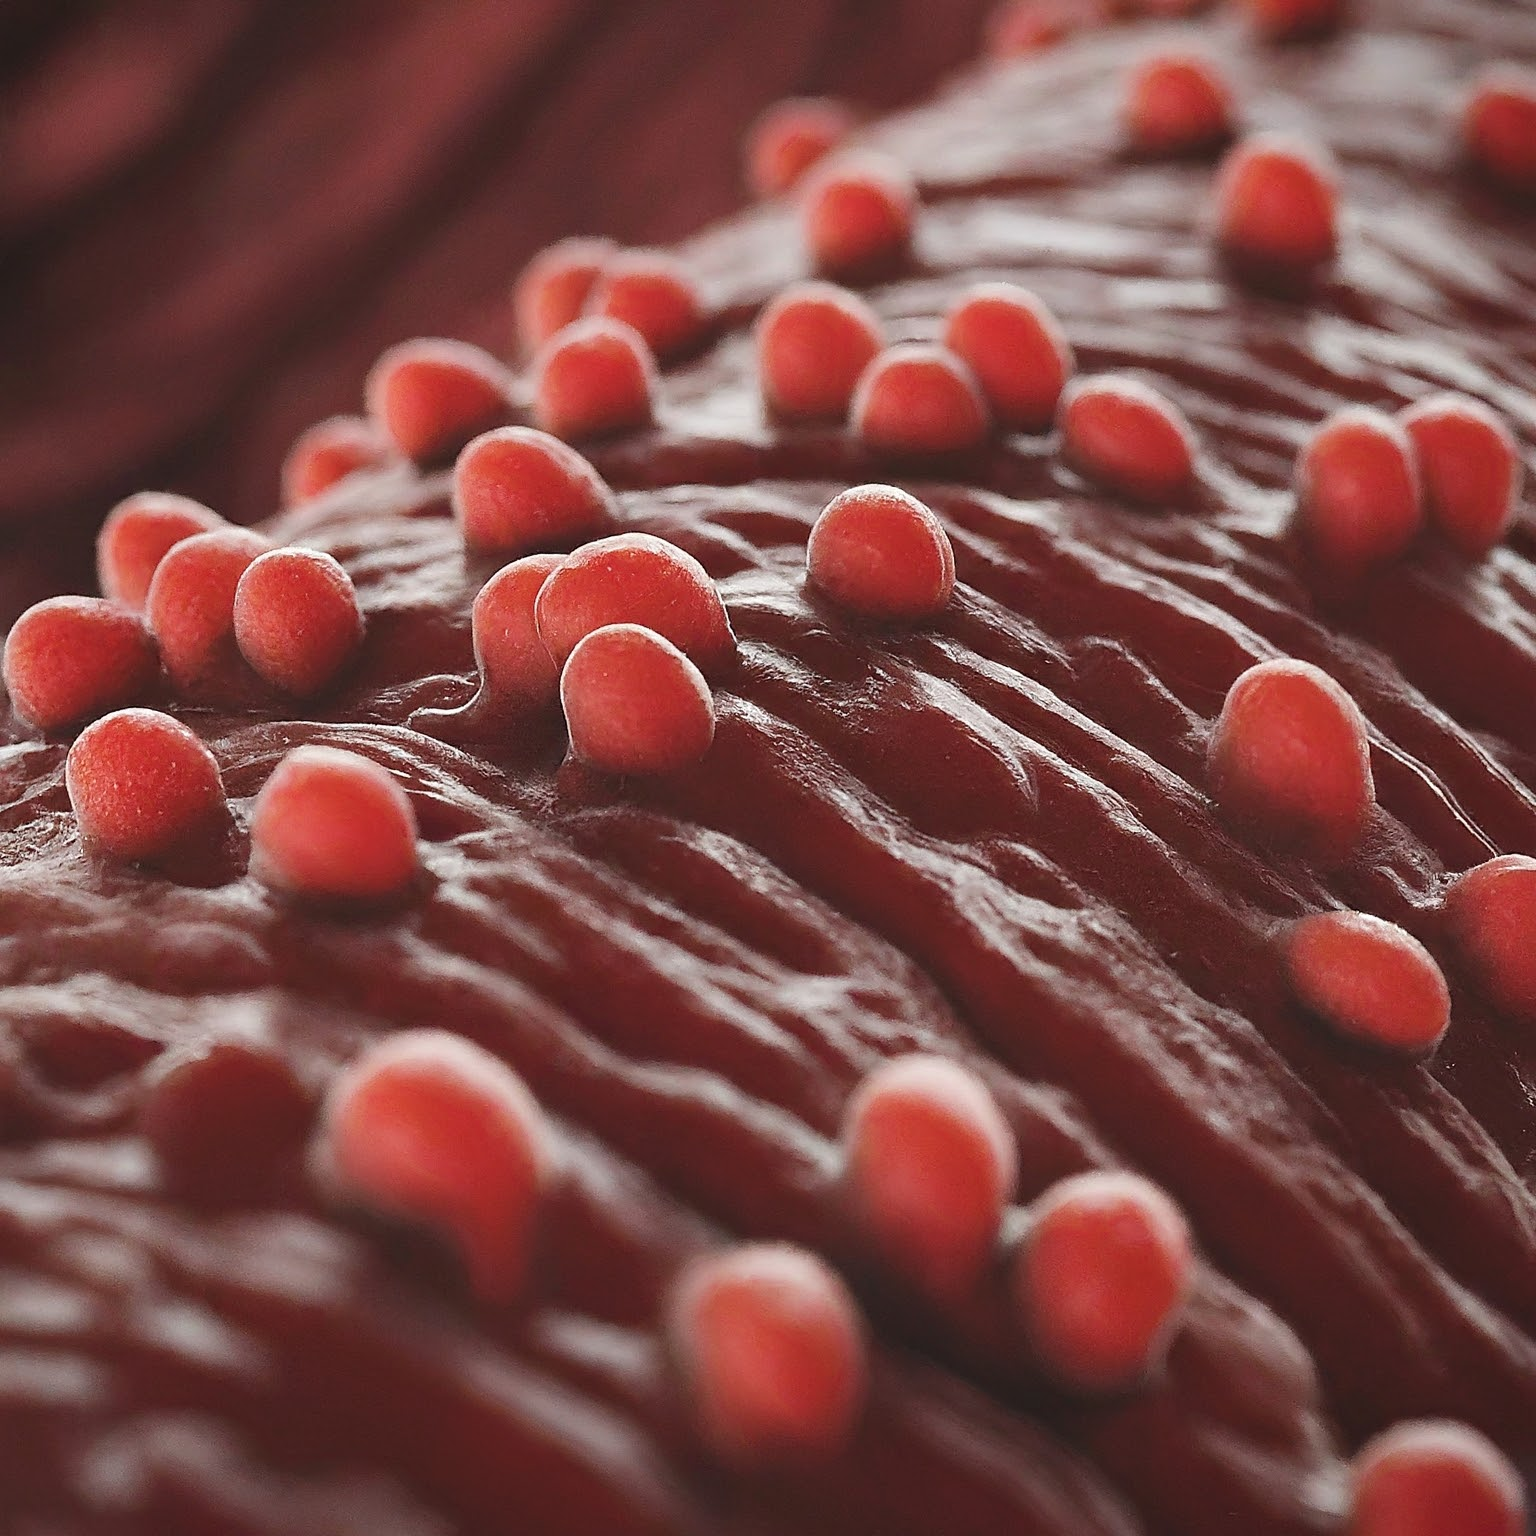
\includegraphics[width=0.15\linewidth]{Gemini_Generated_Image.jpeg}
        \caption{Mechanoreceptor in the Blood Vessels}
        \label{fig:enter-label}
    \end{figure}
    \item When a mechanosensor feels the force, it sends a message inside the cell, like a chemical signal. This is the process of mechanotransduction.
    \item Stem cells also have mechanosensors, just like other cells. These sensors can detect physical forces like stiffness, pressure, and even blood flow.

    \item  \textbf{Mesenchymal stem cells} (MSCs), are being explored for their ability to repair damaged tissues. 
    \newpage
    \item  MSCs are capable of transforming into various cell types like bone, cartilage, or muscle. This makes them ideal for treating damaged tissues.
    \begin{figure}[h]
        \centering
        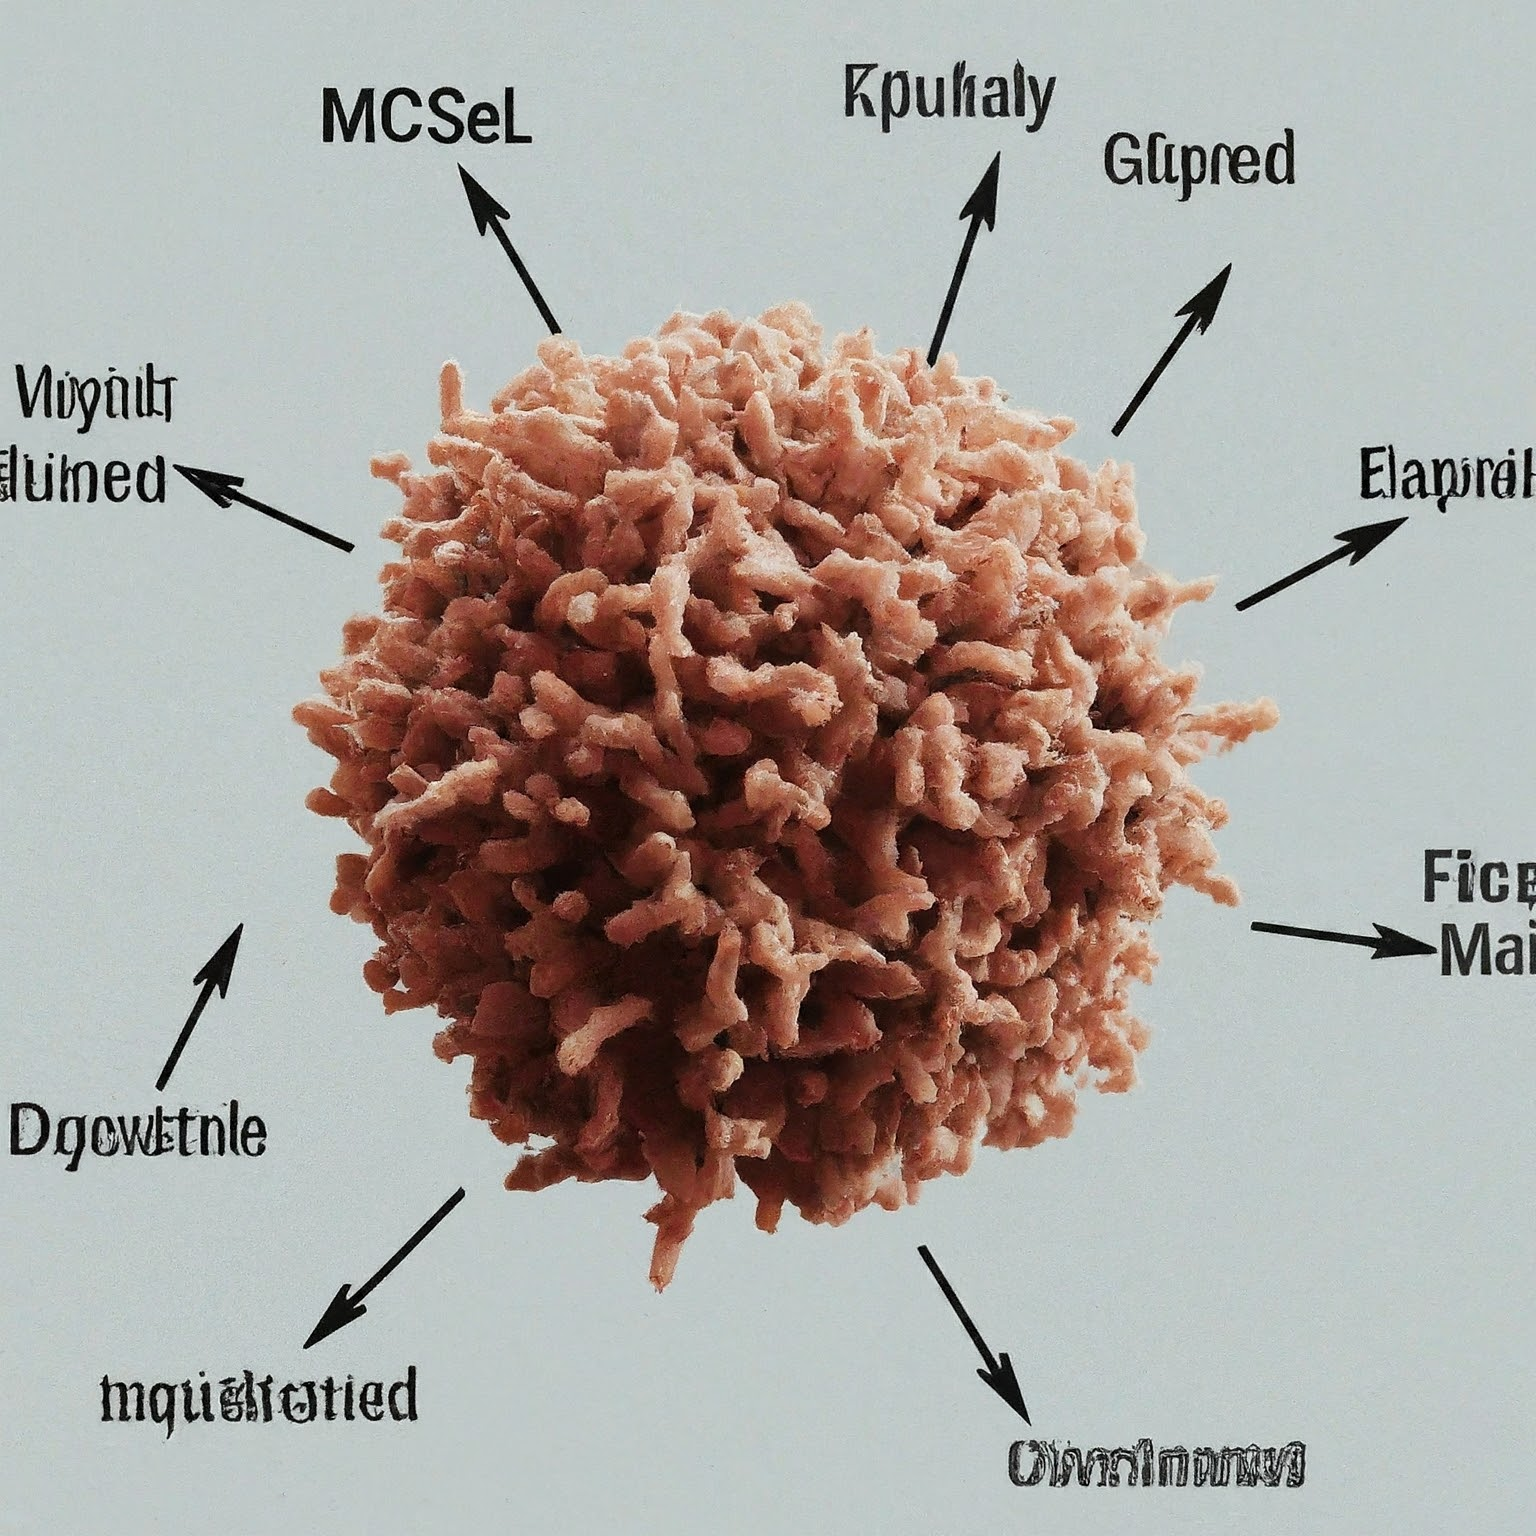
\includegraphics[width=0.15\linewidth]{Gemini_Generated_Image (1).jpeg}
        \caption{MSC Cell}
        \label{fig:enter-label}
    \end{figure}
   \item  Depending on the forces and other factors, the MSCs can differentiate into different cell types:
\begin{enumerate}
\item \textbf{Stiff environment}: Favors bone cell differentiation.
\item \textbf{Flowing environment}:promotes blood vessel cell differentiation.

\end{enumerate}
   \item  By understanding how forces influence MSC differentiation, scientists are developing new treatments for various conditions like:

\begin{enumerate}
\item \textbf{Bone repair}: Using MSCs stimulated by bone-like forces to heal fractures.
\item \textbf{Cartilage regeneration}: Applying controlled forces to guide MSCs into cartilage-forming cells.
\item \textbf{Heart muscle repair}: Mimicking the flow in blood vessels to encourage MSCs into heart muscle cells.
\end{enumerate}
\begin{figure}[h]
    \centering
    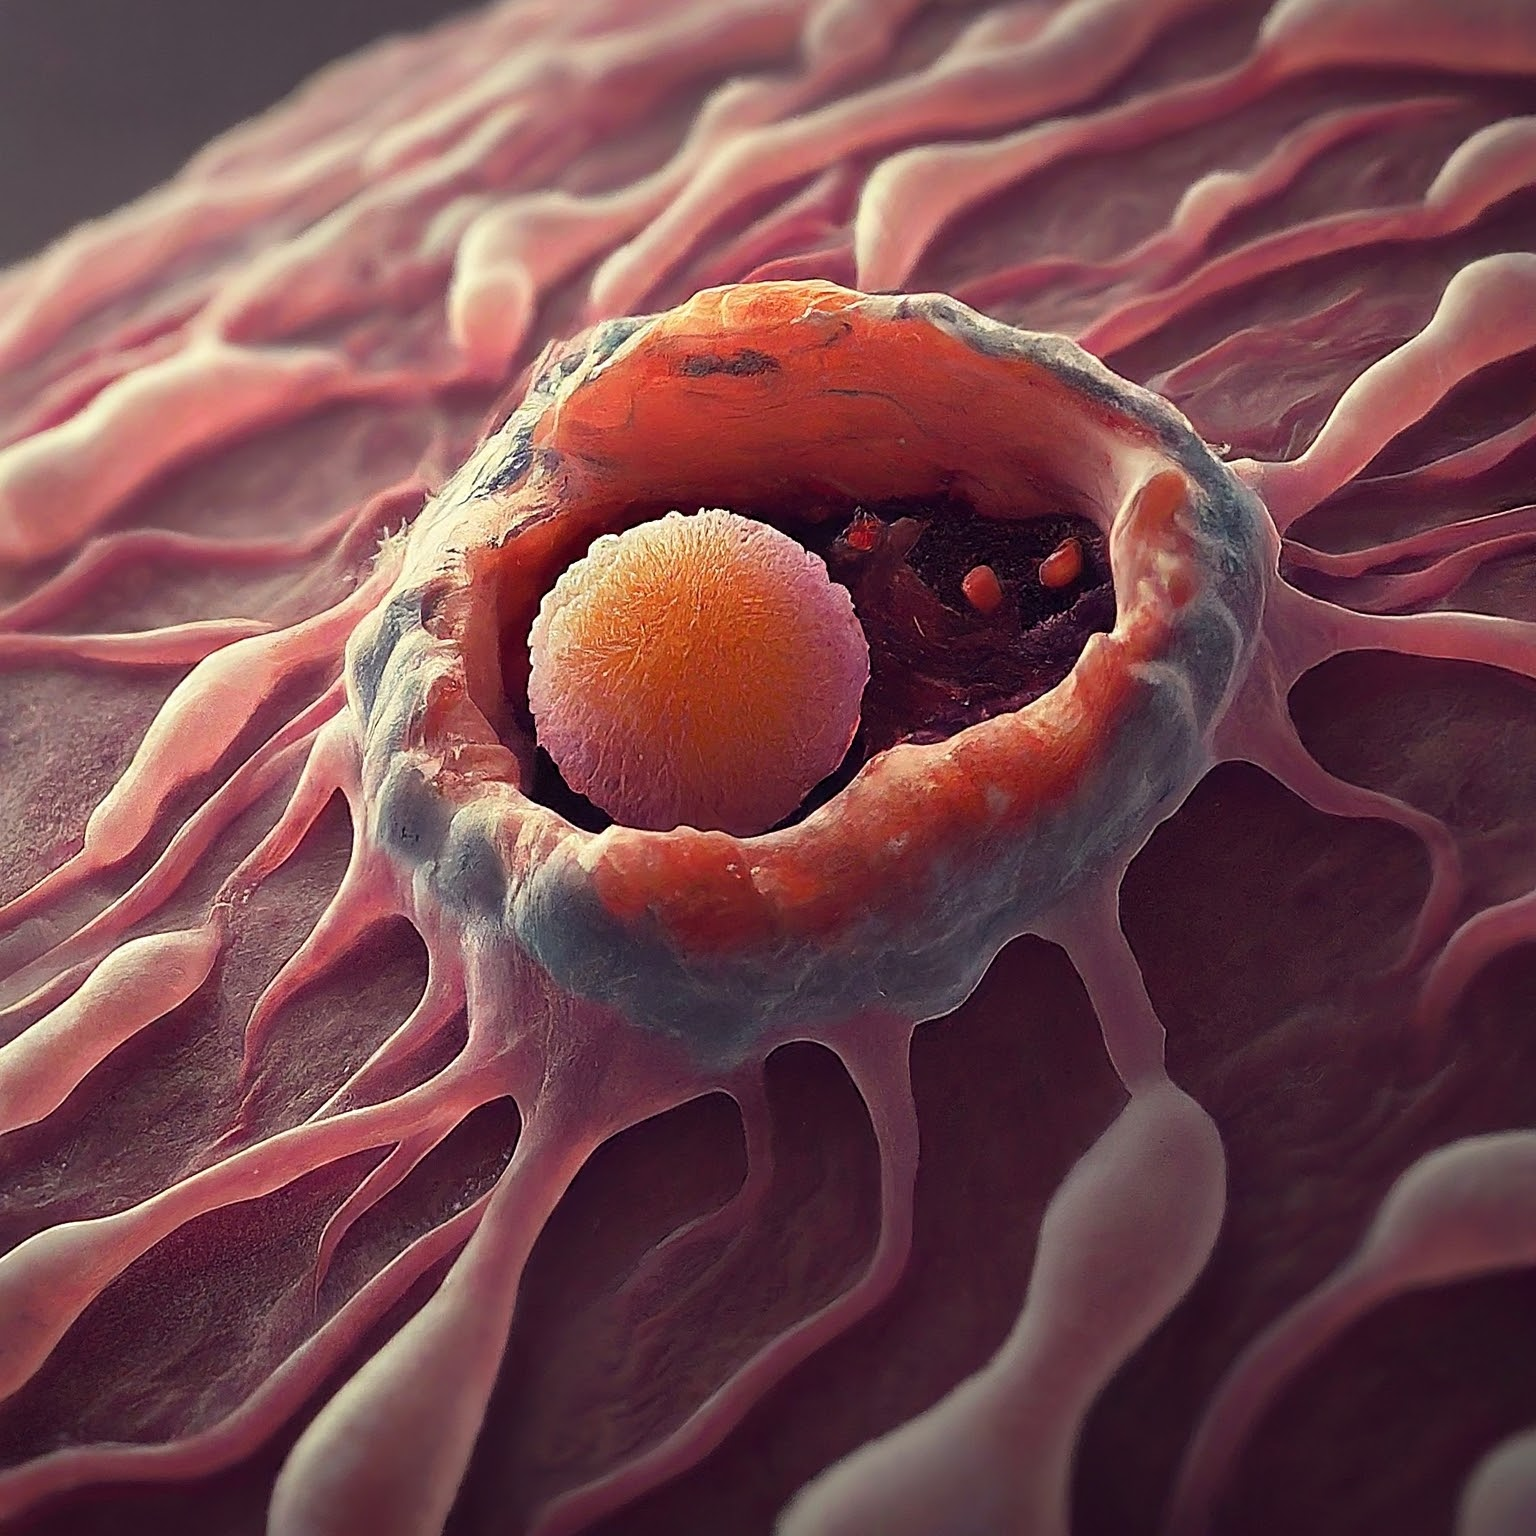
\includegraphics[width=0.15\linewidth]{Gemini_Generated_Image (2).jpeg}
    \caption{repair action of a MSC cell}
    \label{fig:enter-label}
\end{figure}
\end{itemize}
\subsubsection{Conclusion}
In summary, the stiffness of a substrate influences a variety of cell processes, including cell shape, adhesion, migration, differentiation, and proliferation. Cell morphology has recently garnered renewed interest, owing to the possibility that measuring, predicting, and regulating cellular form would be useful in future tissue regeneration
\subsubsection{Reference(Nature Journal)}
1.Raman, N., Imran, S. A. M., Ahmad Amin Noordin, K. B., Zaman, W. S. W. K. & Nordin, F. Mechanotransduction in Mesenchymal Stem Cells (MSCs) Differentiation: A Review. International Journal of Molecular Sciences 23, 4580 (2022).
\newpage
\subsection{YAP/TAZ upstream signals and downstream responses}
\subsubsection{Mechanism}
\begin{itemize}
    \item \textbf{Non-genetic basis of complex behaviors}: Morphogenesis, collective migration, and self-organization in cells are not directly encoded in genes but emerge from interconnected cell networks. (Diagram 1)
\item \textbf{Disease and tissue environment}: Most diseases aren't primarily genetic, but involve "corrupted" tissue environments that drive abnormal cell behavior. (Diagram 2)
\item \textbf{Cancer example}: Even in genetic diseases like cancer, changes in the tissue environment precede or accompany genetic mutations and contribute to aberrant cell behavior.
\item \textbf{YAP/TAZ as Cell Sensors}: These transcriptional regulators act as sensors, allowing cells to "feel" their own shape, polarity, and the surrounding tissue environment.
\item \textbf{Shape and Polarity Control}: The activity of YAP/TAZ is directly controlled by a cell's shape and polarity, which are determined by the cytoskeleton, a network of fibers inside the cell.
\item \textbf{Interlinked Features}: A cell's structure (shape, cytoskeleton) is linked to its metabolism, responsiveness to environmental cues (morphogens, nutrients), and mechanical forces.
\begin{figure}[h]
    \centering
    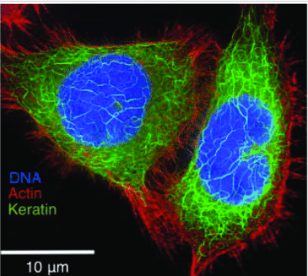
\includegraphics[width=0.15\linewidth]{Screenshot from 2024-02-25 12-32-07.png}
    \caption{Fluorescence micrography  with the parts of a cytoskeleton}
    \label{fig:enter-label}
\end{figure}

\item \textbf{Mechanical Balance}: Cells constantly adjust their internal and external forces to maintain equilibrium.
\item \textbf{ECM rigidity}: Stiffness of the surrounding extracellular matrix influences cell behavior.
\begin{figure}[h]
    \centering
    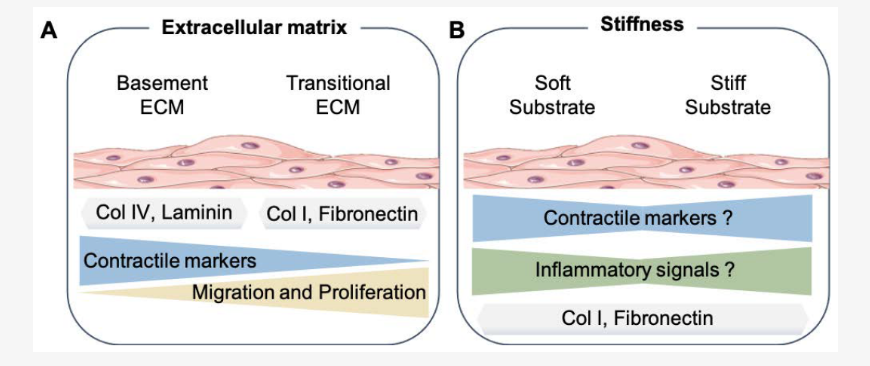
\includegraphics[width=0.5\linewidth]{Screenshot from 2024-02-25 12-38-10.png}
    \caption{Smooth muscle cell mechanical microenvironment}
    \label{fig:enter-label}
\end{figure}
\newpage
\item \textbf{ECM remodeling}: Cells can modify the composition and structure of the surrounding ECM.
\begin{figure}
    \centering
    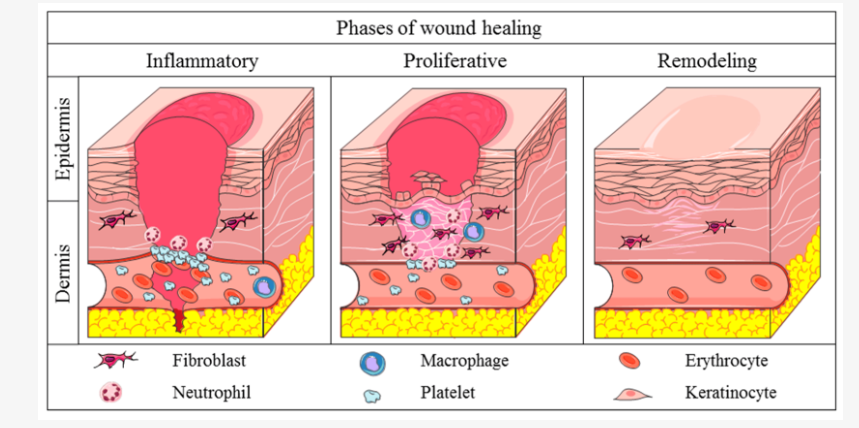
\includegraphics[width=0.4\linewidth]{Screenshot from 2024-02-25 12-45-56.png}
    \caption{Remodelling of ECM skin cells during wound healing}
    \label{fig:enter-label}
\end{figure}
\item YAP/TAZ: Orchestrating Mechanics, Metabolism, and Development
\begin{enumerate}
\item \textbf{YAP/TAZ} : These regulators play a key role in integrating cellular mechanics, metabolism, and developmental signaling.
\item \textbf{Positive Feedback Loop}: YAP/TAZ activity \ create positive feedback systems, amplifying their own mechanical and metabolic signaling.
\item \textbf{Organ development}: Shaping organs during development..
\item \textbf{Disease Link}: YAP/TAZ dysfunction can lead to various diseases like fibrosis, cancer, and atherosclerosis.
\end{enumerate}    
\begin{verbatim}
                Cell Mechanics (Shape, Tension)
                         | 
                         |  
                         v    
                 YAP/TAZ Activation
                         | 
                         |  
                         v    
        Metabolism (Gene Expression, Nutrient Uptake)
                         | 
                         |  
                         v    
        Developmental Signaling (Pathways, Morphogen Signals)
                         | 
                         |  
                         v    
        Cell Response & Adaptation (Growth, Differentiation, Tissue Function)
                         | 
                         |
                         v    
        Positive Feedback Loop (Amplifies YAP/TAZ Activity)
\end{verbatim}
\end{itemize}
\newpage
\subsubsection{Conclusion}
\begin{itemize}
    \item Cytoskeletal organization serves as a key determinant of YAP/TAZ activation in response to tissue-level mechanical forces.
    \item YAP/TAZ impact cellular events, including growth factor responsiveness and metabolism.
    \item Activation of YAP/TAZ can reprogram normal cells into tissue-specific stem or progenitor cells, relevant to regenerative medicine.
    \item The interplay between YAP/TAZ and cell mechanics, as well as their role in cancer and regeneration, presents potential for clinical applications in anti-cancer therapies.
\end{itemize}
\subsubsection{References(Nature Journal)}
\begin{enumerate}
    \item Totaro, A., Panciera, T. \& Piccolo, S. YAP/TAZ upstream signals and downstream responses. Nature Cell Biology vols. 888–899 https://doi.org/10.1038/s41556-018-0142-z (2018).
    \item Hémonnot, C. Y. J. Investigating Cellular Nanoscale with X-rays. Göttingen series in x-ray physics https://doi.org/10.17875/gup2016-996 (2016) doi:10.17875/gup2016-996.
    \item Gushiken, L. F. S., Beserra, F. P., Bastos, J. K., Jackson, C. J. \& Pellizzon, C. H. Cutaneous Wound Healing: An Update from Physiopathology to Current Therapies. Life vol. 665 https://doi.org/10.3390/life11070665 (2021).
\end{enumerate}
\subsection{Mechanosensory Signaling in Astrocytes}
\subsubsection{Mechanism}
\begin{itemize}
    \item \textbf{Astrocytes} are star-shaped cells in the brain are known for their mechanosensitivity, meaning they can sense and respond to mechanical forces
    \item \textbf{Sensitive to pressure}: Astrocytes can detect even slight changes in pressure, especially drops in cerebral perfusion pressure (CPP), which signifies reduced blood flow to the brain.
    \begin{figure}[h]
        \centering
        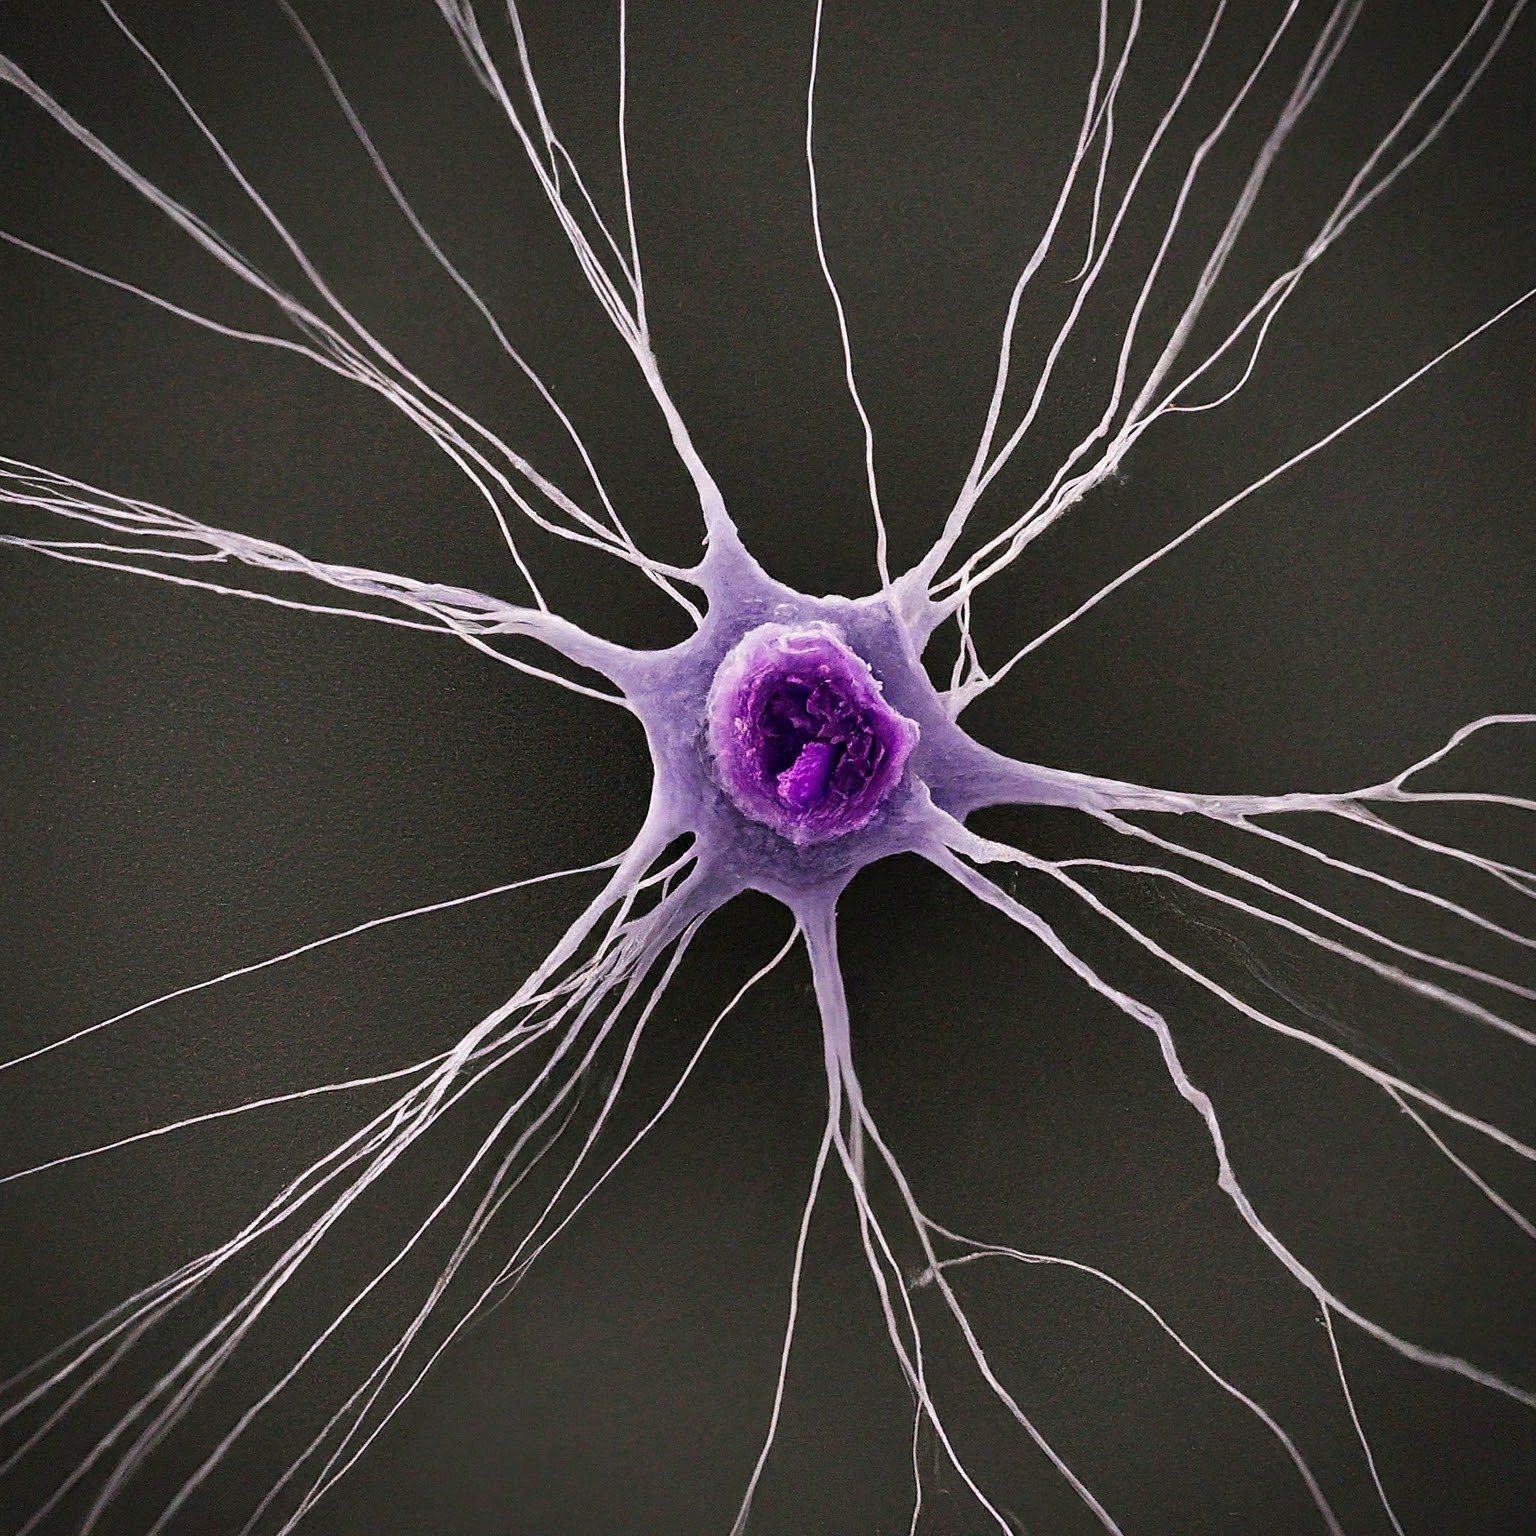
\includegraphics[width=0.15\linewidth]{Gemini_Generated_Image (3).jpeg}
        \caption{astrocytes}
        \label{fig:enter-label}
    \end{figure}
\item Mechanosensitive: Brainstem astrocytes respond to mechanical stimulation, potentially mimicking changes in blood flow pressure.
\item \textbf{Calcium Signaling}: This stimulation triggers an increase in calcium (Ca2+) within the cells, suggesting activation of signaling pathways.
\item \textbf{Connexin Channels}: Blocking these channels, specifically CX 43, prevents the calcium response, indicating their involvement in mechanosensing.
\item Key Findings in Cx43 Knockout Mice:
\begin{itemize}
    \item 
\textbf{Acute Pressure Response}: Despite lacking Cx43, these mice responded normally to sudden increases in intracranial pressure, suggesting alternative pathways for immediate heart rate adjustments.
\item
\textbf{Chronic Perfusion Effects}: However, Cx43 deficiency led to consistently lower heart rates at various cerebral perfusion levels. This supports the hypothesis that Cx43 channels play a role in maintaining higher heart rates under normal conditions.

\item \textbf{Astrocyte Signaling}: This suggests Cx43 channels in astrocytes might release signaling molecules that excite nerve circuits controlling heart rate.
\end{itemize}
\begin{figure}[h]
    \centering
    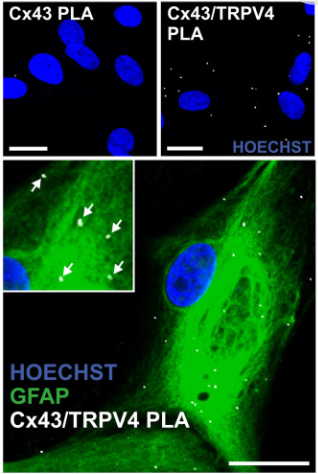
\includegraphics[width=0.15\linewidth]{Screenshot from 2024-02-25 14-19-52.png}
    \caption{interaction between Cx43 and TRPV4 channels}
    \label{fig:enter-label}
\end{figure}
\item To function as intracranial baroreceptors, astrocytes must possess a specialized membrane mechanism that makes them exquisitely sensitive to mechanical stimuli. 
\item This study shows that opening of connexin 43 (Cx43) hemichannels leading to the release of ATP is the key central event underlying mechanosensory Ca2+ responses in astrocytes.
\end{itemize}
\subsubsection{Conclusion}
\begin{itemize}
\item Mechanosensory signaling in brainstem astrocytes was studied using two controlled mechanical stimulation methods.
\item Ca2+ responses in individual astrocytes were robust and reproducible with timed ejections of extracellular media.
\item Mechanical stimulation-induced Ca2+ signals were significantly reduced by pharmacological inhibition of connexin/pannexin channels, gap junctions, TRPV4 channels, or P2Y1 receptors..
\item This study provides insights into the mechanosensitive behavior of brainstem astrocytes and identifies key membrane targets involved in their Ca2+ signaling.
\subsubsection{References(Nature Journal)}
1.Turovsky, E. A. et al. Mechanosensory Signaling in Astrocytes. The Journal of Neuroscience vols. 9364–9371 https://doi.org/10.1523/jneurosci.1249-20.2020 (2020).
\newpage
\end{itemize}
\subsection{Cx43 and mechanotransduction in bone}
\subsubsection{Mechanism}
\begin{itemize}
\item \textbf{Bone adapts to changes in mechanical stimuli} by adjusting bone formation (by osteoblasts) and resorption (by osteoclasts) to maintain optimal bone mass.
\item \textbf{Osteocytes sense mechanical forces} and produce cytokines that control the activity of osteoblasts and osteoclasts.
\item \textbf{Connexin channels} (Cxs), especially Cx43, are thought to be important for this communication.
\item \textbf{Mice lacking Cx43} in osteoblasts and osteocytes show an unexpected response to mechanical stimulation:
\begin{itemize}
\item \textbf{Increased bone formation} in response to loading (opposite of what was expected).
\item \textbf{Decreased bone loss} in response to unloading (opposite of what was expected).
\end{itemize}
\item This suggests that \textbf{Cx43 channels may not be essential} for the initial response to mechanical stimuli, but may play a role in regulating the long-term consequences.
\item Connexin channels can also form hemichannels, which are open to the extracellular space.
\item Hemichannels have been shown to mediate communication between cells and the extracellular milieu.
\item Cx43 hemichannels were first reported in osteoblastic and osteocytic cell lines in the early 2000s.
\item Removal of extracellular calcium can induce the opening of Cx43 hemichannels in osteoblastic and osteocytic cells.
\item Opening of Cx43 hemichannels is required for the anti-apoptotic effect of bisphosphonates.
\begin{figure}[h]
    \centering
    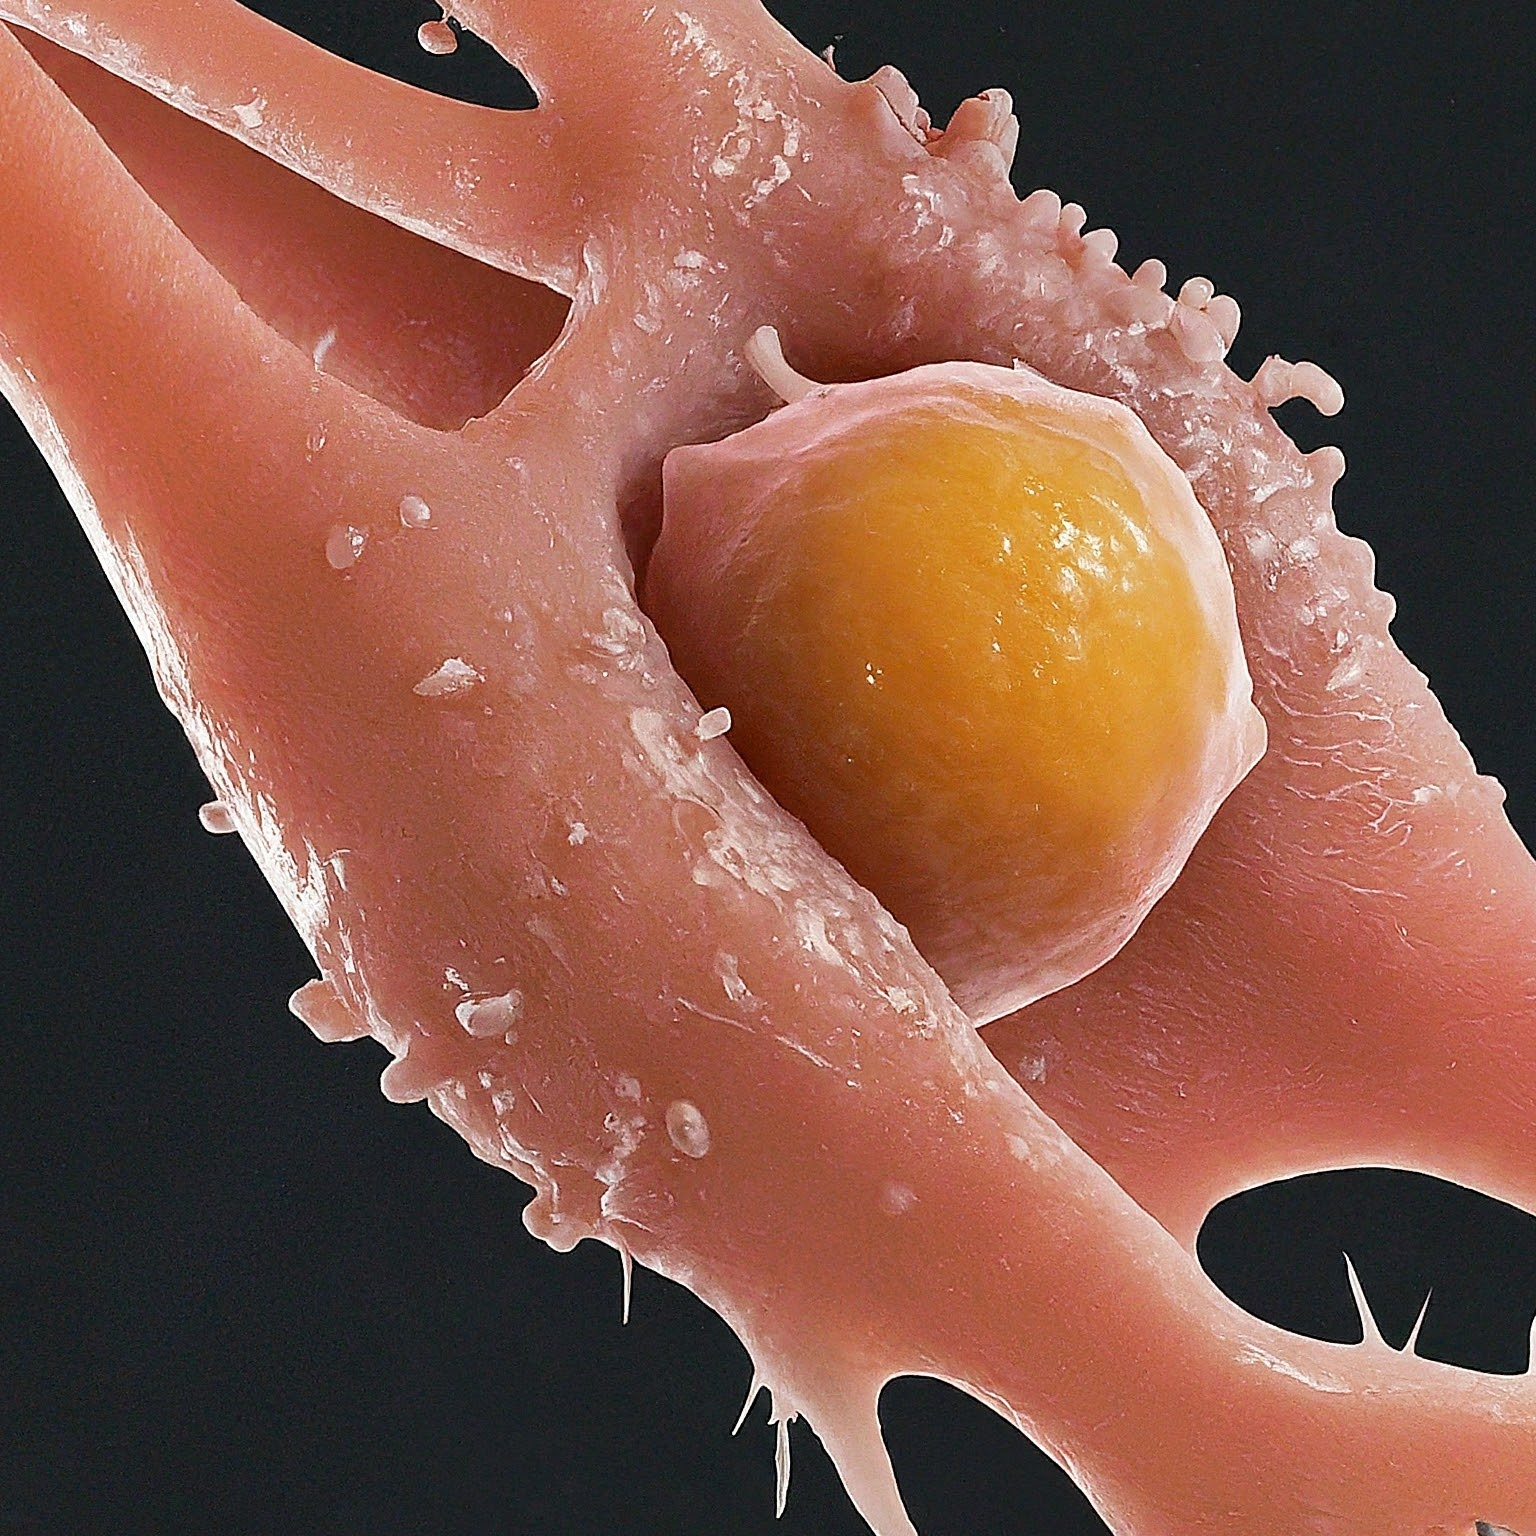
\includegraphics[width=0.15\linewidth]{Gemini_Generated_Image (4).jpeg}
    \caption{Conexin Hemichannels}
    \label{fig:enter-label}
\end{figure}
\end{itemize}
\subsubsection{Conclusion}
Cx43 hemichannels appear to be required for the survival effect of mechanical stimulation mediated by PGE2 in vitro, the role of the connexin in vivo is not so direct. Thus, mice lacking Cx43 in osteoblastic cells do not show a cancellous bone phenotype under normal ambulatory conditions.
\subsubsection{Reference(Nature Journal)}
1.Plotkin, L. I., Speacht, T. L. \& Donahue, H. J. Cx43 and Mechanotransduction in Bone. Current Osteoporosis Reports vols. 67–72 https://doi.org/10.1007/s11914-015-0255-2 (2015).
\newpage
\subsection{The Involvement of Cx43 in JNK1/2-Mediated Endothelial Mechanotransduction and Human Plaque Progression}
\begin{itemize}
\item  Atherosclerosis: A disease characterized by the buildup of plaque in arteries, often starting at bifurcations where blood flow is irregular.

 \begin{figure}[h]
    \centering
    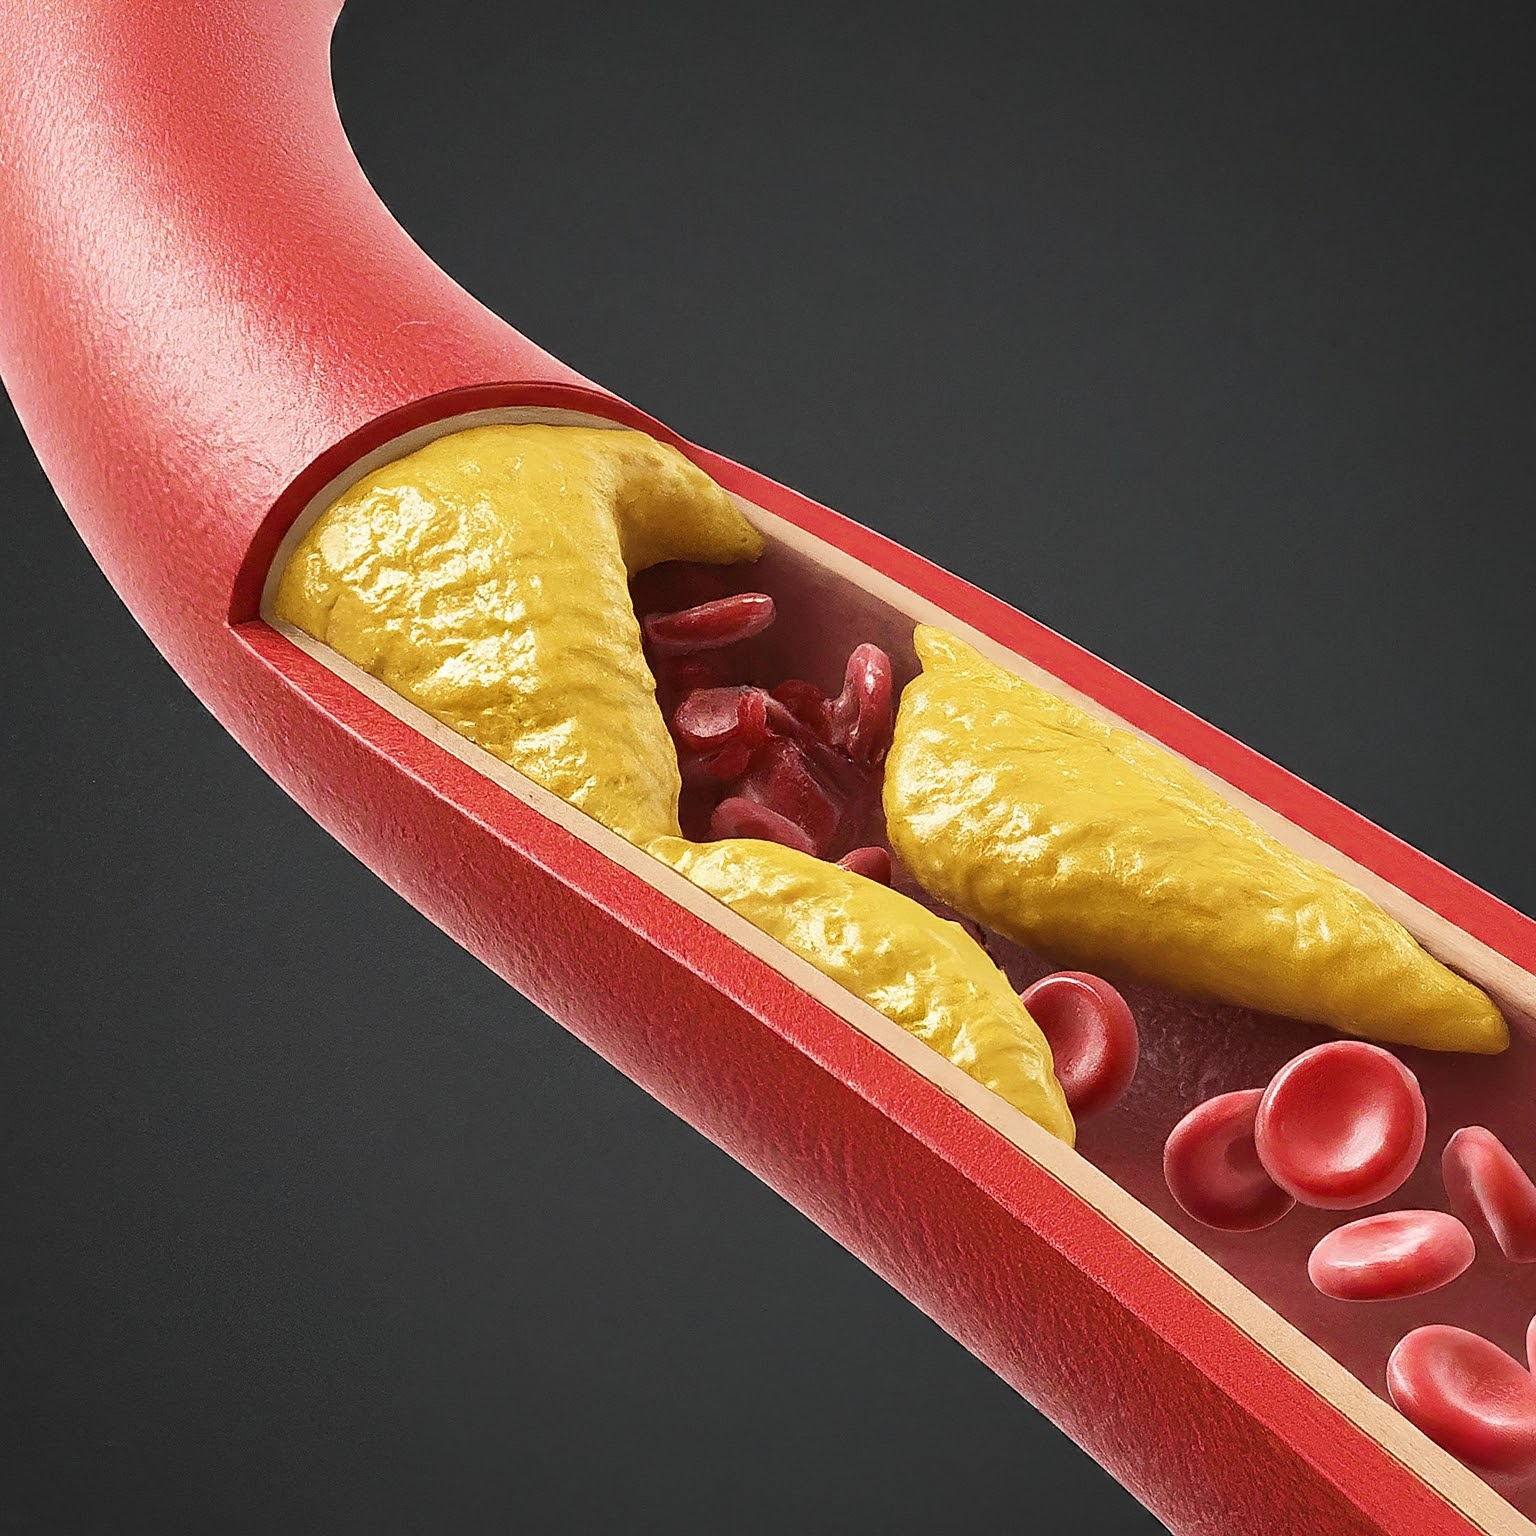
\includegraphics[width=0.15\linewidth]{Gemini_Generated_Image (5).jpeg}
    \caption{Atherosclerosis}
    \label{fig:enter-label}
\end{figure}

 \item Shear stress (SS): The force exerted by blood flow on the endothelium, the inner lining of arteries.
 
\item MAPKs: Mitogen-activated protein kinases, signaling molecules involved in cell growth and proliferation.
 \item Connexins (Cxs): Proteins that form gap junctions, channels that allow communication between cells.
\item Human umbilical vein endothelial cells (HUVECs): Cells used in the study to model the endothelium.
\item HUVECs were exposed to different levels of SS ("mechanical stimulation").
\item \textbf{Results:
}
\begin{enumerate}
    \item 
SS activated MAPKs and downstream signaling in HUVECs.
\item SS increased the expression of certain Cxs.
\item There was an interaction between SS and inflammatory stimulation on Cx expression and signaling.
\end{enumerate}
\item Inhibition of JNK1/2 pathway: Reduced Cx43 expression and prevented inflammation in atherosclerotic lesions in mice.
Human carotid plaques:
\item More Cx43+ cells found in vulnerable (prone to rupture) plaques compared to stable ones.
\item Number of Cx43+ cells correlated with increased inflammation, blood vessel growth, and lipid core size (unstable plaque features).
\item Number of Cx43+ cells inversely correlated with fibrous cap thickness (plaque stability feature).
Overall:
\end{itemize}
\subsubsection{Conclusion}
\begin{itemize}
\item Cx43 expression linked to plaque progression and instability.
\item JNK1/2 pathway may control Cx43 levels and be a potential target for treating atherosclerosis.
\item First study to show Cx43 expression in human carotid plaques and its association with plaque vulnerability.
\end{itemize}
\subsubsection{Reference(Nature Journal)}
1.Tauchi, M. et al. The Involvement of Cx43 in JNK1/2-Mediated Endothelial Mechanotransduction and Human Plaque Progression. International Journal of Molecular Sciences vol. 1174 https://doi.org/10.3390/ijms24021174 (2023).
\newpage
\section{\textit{Important Conclusions}}
\begin{itemize}
\item Mechanosensory signaling in brainstem astrocytes was studied using two controlled mechanical stimulation methods.
\item Cx43 expression linked to plaque progression and instability.
\end{itemize}

\end{document}
